\appendix
\chapter{UML Models}

\section{Business Class Diagram}

\begin{center}
\begin{figure}[h!]
\scalebox{0.65}{
\begin{tikzpicture}
%\begin{umlpackage}{p}
%\begin{umlpackage}{sp1}

\umlclass[x=-5]{Sendable}{
  - trackers : list<tracker> \\
  - seeders  : list<seeder> \\
  - speed    : double
}{
  + start() : void \\
  + stop() : void \\
  + pause() : void \\
  + resume() : void
}

\umlclass[x=3]{FileManager}{
  - list<File>
}{
  + remove(File file) : void \\
  + add(File file) : File \\
  + rename(File file) : File \\
  + sort() : void \\
  + search(File file) : list<File> \\
}

\umlclass[x=3, y=-6]{File}{
  - name : String \\
  - date : String \\
  - extension : String \\
  - size : double \\
  - visible : bool \\
}{
  + setVisibility(bool value) : void \\
  + isVisible() : bool \\
  + setName(String name) : void \\
  + getSize() : double \\
  + getDate() : String \\
  + getName() : String
}

\umlclass[x=4, y=-11]{Media}{
  - length : double \\
}{}

\umlclass[x=-7, y=-4]{Download}{
  - percentage : double
}{}

\umlclass[x=-3, y=-4]{Upload}{
  - amount : double
}{}

\umlclass[x=-5, y=-6]{Stream}{
  - length : double
}{}

\umlclass[x=-5, y=-10.5]{DownloadManager}{
  - downloaded : double \\
  - uploaded : double \\
  - downloads : list<Download> \\
  - uploads : list<Uploads>
}{
  + startDownload(String link) : void \\
  + stopDownload(String link) : void \\
  + pauseDownload(String link) : void \\
  + resumeDownload(String link) : void \\
  + startUpload(String name) : void \\
  + stopUpload(String name) : void
}

\umlclass[x=2, y=-14]{MediaPlayer}{
}{
  + open(Media file) : void \\
  + open(Stream stream) : void
}

\umlaggreg[mult1=1, mult2=1, pos=0.8, angle1=30, angle2=60]{Sendable}{File}
\umlaggreg[mult1=1, mult2=*]{FileManager}{File}

\umlinherit{Download}{Sendable}
\umlinherit{Upload}{Sendable}
\umlinherit{Stream}{Sendable}

\umlinherit{Media}{File}

\umlVHVaggreg[mult1=1, mult2=*]{DownloadManager}{Upload}
\umlVHVaggreg[mult1=1, mult2=*]{DownloadManager}{Download}

\umlVHassoc{MediaPlayer}{Stream}
\umlVHassoc{Media}{MediaPlayer}

\end{tikzpicture}}
\caption{Part of the class diagram. This part only shows the business classes comprehensible for end-users.}
\label{fig:business_class}
\end{figure}
\end{center}

\section{Use Case Dynamic Models}
\label{sec:req_dynamic_models}
\begin{figure}[h!]
\scalebox{1}{
\begin{tikzpicture}
\begin{umlseqdiag}
\umlactor{User}
\umlobject[x=5]{Samsung App Interface}
\umlobject[x=10]{DownloadManager}
\begin{umlcall}[op={goToSettings()}, with return, padding=3]{User}{Samsung App Interface}
\begin{umlcall}[op={getSettings()}, with return]{Samsung App Interface}{DownloadManager}
\end{umlcall}
\end{umlcall}
\begin{umlcall}[op={setSpeeds(dspeed, uspeed)}, padding=3, with return]{User}{Samsung App Interface}

\begin{umlcall}[op={setSpeeds(dspeed, uspeed)}, padding=3, with return]{Samsung App Interface}{DownloadManager}
\end{umlcall}
\end{umlcall}
\end{umlseqdiag}
\end{tikzpicture}
}
\caption{Use Case 1: Limit upload/download speeds.}
\label{fig:req_seq1}
\end{figure}

\begin{figure}[h!]
\scalebox{0.8}{
\begin{tikzpicture}
\begin{umlseqdiag}
\umlactor{User}
\umlobject{Samsung App Interface}
\umlobject{FileManager}
\umlobject{MediaPlayer}
\umlmulti{File}

\begin{umlcall}[op={browse}, with return, padding=3]{User}{Samsung App Interface}
	\begin{umlcall}[op={getFiles()}, with return, padding=3]{Samsung App Interface}{FileManager}
		\begin{umlcall}[op={get()}, with return, padding=3]{FileManager}{File}
		\end{umlcall}
	\end{umlcall}
\end{umlcall}

\begin{umlfragment}[type=alt, label=Update, inner xsep=5]
\begin{umlcall}[op={update}, with return]{User}{Samsung App Interface}
	\begin{umlcall}[op={update(int file\_id)}, with return]{Samsung App Interface}{FileManager}
		\begin{umlcall}[op={update()}, with return]{FileManager}{File}
		\end{umlcall}
	\end{umlcall}
\end{umlcall}

\umlfpart [Delete]
\begin{umlcall}[op={delete}, with return]{User}{Samsung App Interface}
	\begin{umlcall}[op={delete(int file\_id)}, with return]{Samsung App Interface}{FileManager}
		\begin{umlcall}[op={destroy()}, with return]{FileManager}{File}
		\end{umlcall}
	\end{umlcall}
\end{umlcall}

\umlfpart[Move]
\begin{umlcall}[op={move}, with return]{User}{Samsung App Interface}
	\begin{umlcall}[op={move(string location, int file\_id)}, with return]{Samsung App Interface}{FileManager}
		\begin{umlcall}[op={changeLocation(string location)}, with return]{FileManager}{File}
		\end{umlcall}
	\end{umlcall}
\end{umlcall}

\umlfpart[Play]
\begin{umlcall}[op={play}, with return]{User}{Samsung App Interface}
	\begin{umlcall}[op={play(int file\_id)}, with return]{Samsung App Interface}{MediaPlayer}
		\begin{umlcall}[op={play()}, with return]{MediaPlayer}{File}
		\end{umlcall}
	\end{umlcall}
\end{umlcall}

\end{umlfragment}
\end{umlseqdiag}
\end{tikzpicture}
}
\caption{Use Cases 2 to 6: Basic browsing and file manipulation}
\label{fig:req_seq2}
\end{figure}

\begin{figure}[h!]
\scalebox{0.9}{
\begin{tikzpicture}
\begin{umlseqdiag}
\umlactor[y=1]{User}
\umlobject[y=1, x=3]{Samsung App Interface}
\umlobject[y=1, x=7]{FileManager}
\umlmulti[y=1, x=12]{File}

\begin{umlcall}[op={change visbility}]{User}{Samsung App Interface}
\end{umlcall}

\begin{umlfragment}[type=alt, label=visible, inner xsep=5]

\begin{umlcall}[op={changeVisibility(file, true)}, with return]{Samsung App Interface}{FileManager}
		\begin{umlcall}[op={visible(true)}, with return]{FileManager}{File}
		\end{umlcall}
\end{umlcall}

\umlfpart[invisible]

\begin{umlcall}[op={changeVisibility(file, false)}, with return]{Samsung App Interface}{FileManager}
		\begin{umlcall}[op={visible(false)}, with return]{FileManager}{File}
		\end{umlcall}
\end{umlcall}

\end{umlfragment}

\end{umlseqdiag}
\end{tikzpicture}
}
\caption{Use Case 7: Change File Visibility}
\label{fig:req_seq3}
\end{figure}

\begin{figure}[h!]
\scalebox{0.8}{
\begin{tikzpicture}
\begin{umlseqdiag}
\umlactor{User}
\umlobject{Samsung App Interface}
\umlobject{FileManager}
\umlobject{DownloadManager}
\umlmulti{File}

\begin{umlcall}[op={goToSearch}, with return, padding=3]{User}{Samsung App Interface}
\end{umlcall}

	\begin{umlfragment}[type=alt, label=Local, inner xsep=5]
		\begin{umlcall}[op={searchLocal(file)}, with return]{User}{Samsung App Interface}
			\begin{umlcall}[op={search(file)}, with return]{Samsung App Interface}{FileManager}
				\begin{umlcall}[op={get()}, with return]{FileManager}{File}
				\end{umlcall}	
			\end{umlcall}
		\end{umlcall}

	\umlfpart [Online]
\begin{umlcall}[op={searchOnline(file)}, with return]{User}{Samsung App Interface}
	\begin{umlcall}[op={search(file)}, with return]{Samsung App Interface}{DownloadManager}
		\begin{umlcall}[op={get()}, with return]{DownloadManager}{File}
		\end{umlcall}
	\end{umlcall}
\end{umlcall}

	
	\end{umlfragment}

\end{umlseqdiag}
\end{tikzpicture}
}
\caption{Use Cases 8 to 10: Search.}
\label{fig:req_seq4}
\end{figure}

\begin{figure}[h!]
\scalebox{1}{
\begin{tikzpicture}
\begin{umlseqdiag}
\umlactor{User}
\umlobject{Samsung App Interface}
\umlobject{DownloadManager}
\umlobject{Stream}

\begin{umlcall}[op={play}]{User}{Samsung App Interface}
\end{umlcall}

\begin{umlcall}[op={playStream(string tracker)}]{Samsung App Interface}{DownloadManager} 
	\begin{umlcall}[op={start()}]{DownloadManager}{Stream} 
	\end{umlcall}
\end{umlcall}

\end{umlseqdiag}
\end{tikzpicture}
}
\caption{Use Case 11: Stream File.}
\label{fig:req_seq5}
\end{figure}

\begin{figure}[h!]
\scalebox{1}{
\begin{tikzpicture}
\begin{umlseqdiag}
\umlactor{User}
\umlobject{Samsung App Interface}
\umlobject{DownloadManager}

\begin{umlcall}[op={download}]{User}{Samsung App Interface}  
\end{umlcall}

\umlcreatecall[class=Download]{Samsung App Interface}{download} 

\begin{umlcall}[op={add(download)}]{Samsung App Interface}{DownloadManager} 
	\begin{umlcall}[op={start()}]{DownloadManager}{download} 
	\end{umlcall} 
\end{umlcall}

\end{umlseqdiag} 
\end{tikzpicture}
}
\caption{Use Case 12: Download File.}
\label{fig:req_seq6}
\end{figure}

\begin{figure}[h!]
\scalebox{1}{
\begin{tikzpicture}
\begin{umlseqdiag}
\umlactor{User}
\umlobject{Samsung App Interface}
\umlobject{FileManager}

	\begin{umlcall}[op={sortName()}, with return]{User}{Samsung App Interface}
		\begin{umlcall}[op={sortName()}, with return]{Samsung App Interface}{FileManager}
		\end{umlcall}
	\end{umlcall}
	
\begin{umlfragment}[type=alt, label=Size, inner xsep=5]
	\begin{umlcall}[op={sortSize(), with return}]{User}{Samsung App Interface}
		\begin{umlcall}[op={sortSize()}, with return]{Samsung App Interface}{FileManager}
		\end{umlcall}
	\end{umlcall}
		
	\umlfpart [Type]
	\begin{umlcall}[op={sortType(), with return}]{User}{Samsung App Interface}
		\begin{umlcall}[op={sortType()}, with return]{Samsung App Interface}{FileManager}
		\end{umlcall}
	\end{umlcall}
		
	\umlfpart [Date]
	\begin{umlcall}[op={sortDate(), with return}]{User}{Samsung App Interface}
		\begin{umlcall}[op={sortDate()}, with return]{Samsung App Interface}{FileManager}
		\end{umlcall}
	\end{umlcall}
\end{umlfragment}

\end{umlseqdiag}
\end{tikzpicture}
}
\caption{Use Cases 13 to 17: Sort Files.}
\label{fig:req_seq7}
\end{figure}

\clearpage

\section{Class diagram}

\begin{center}
\begin{figure}[h!]
\scalebox{1}{
\begin{tikzpicture}
%\begin{umlpackage}{p}
%\begin{umlpackage}{sp1}

\umlclass[x=-10]{Download}{
  - tracker : char* \\
  - id : int \\
  - seeders : int \\
  - peers : int \\
  - ratio : double \\
  - download\_speed : double \\
  - size : double \\
  - upload\_speed : double \\
  - download\_percentage : double \\
  - upload\_amount : double \\
  - is\_visible : bool \\
  - status : Status
}{
  + start() : void \\
  + resume() : void \\
  + pause() : void \\
  + setVisible(bool visible) : void
}

\umlclass[x=-1.5, y=-12]{Stream}{
  - tracker : char*
}{
  + start() : void \\
  + resume() : void \\
  + pause() : void \\
  + stop() : void
}
\umlclass[x=-10, y=-12]{DownloadManager}{
  - downloaded : double \\
  - uploaded : double \\
  - downloads : list<Download> \\
  - uploads : list<Download> \\
}{
  + getInstance() : void \\
  + startStreaming(string tracker) : void \\
  + stopStreaming() : void \\
  + add(Download download) : void \\
  + setVisible(Download download) : void \\
  + setUnvisible(Download download) : void \\
  + resumeDownload(Download download) : void \\
  + removeFromList(int download\_id) : void \\
  + removeFromDisk(int download\_id) : void \\
  + setSpeed(double dspeed, double uspeed)
}

\umlclass[x=-3, y=-6]{HttpServer}{
}{
  + InstallHTTPGateway() : bool \\
  + sendResponse() : void \\
  + sendXMLResponse() : void \\
  + handle\_request(struct evhttp\_request *req, void *arg) : void \\
}

\umlclass[x=-0.5, y = 2]{SearchEngine}{
}{
  + search(char* filename) : void \\
  + getResults() : char*
}

\umlVHassoc[mult1=1, mult2=*]{HttpServer}{Download}
\umlassoc[mult1=1, mult2=1]{HttpServer}{DownloadManager}
\umlVHassoc[mult1=1, mult2=1]{SearchEngine}{HttpServer}

\umlaggreg[mult1=1, mult2=*]{DownloadManager}{Download}
\umlaggreg[mult1=1, mult2=1]{DownloadManager}{Stream}

\end{tikzpicture}}
\caption{Class diagram of the webserver subsystem.}
\label{fig:class_server}
\end{figure}
\end{center}

\section{Dynamic models}

\begin{figure}[h!]
\scalebox{1}{
\begin{tikzpicture}
\begin{umlseqdiag}
\umlactor{Samsung SDK client}
\umlobject[x=5]{HttpServer}
\umlobject[x=8]{DownloadManager}
\begin{umlcall}[op={sendRequest(add download)}, with return, padding=3]{Samsung SDK client}{HttpServer}
	\begin{umlcall}[op={add(download)}, with return, padding=3]{HttpServer}{DownloadManager}
		\umlcreatecall[class=Download]{DownloadManager}{download}
		\begin{umlcall}[op={setStatus(READY)}, padding=3]{DownloadManager}{download}
		\end{umlcall}
		\begin{umlcall}[op={push(download)}, padding=3]{DownloadManager}{DownloadManager}
		\end{umlcall}
	\end{umlcall}
\end{umlcall}
\end{umlseqdiag}
\end{tikzpicture}
}
\label{fig:seq1}
\caption{Add download}
\end{figure}

\begin{figure}[h!]
\scalebox{0.7}{
\begin{tikzpicture}
\begin{umlseqdiag}
\umlactor{Samsung SDK client}
\umlobject[x=5]{HttpServer}
\umlobject[x=8]{DownloadManager}
\umlobject[x=12]{Download}
\umlobject[x=18]{Swift}
\begin{umlcall}[op={sendRequest(start download)}, with return, padding=3]{Samsung SDK client}{HttpServer}
	\begin{umlcall}[op={start(download)}, with return, padding=3]{HttpServer}{DownloadManager}
		\begin{umlcall}[op={get(download)}, padding=3]{DownloadManager}{DownloadManager}
		\end{umlcall}
		
		\begin{umlcall}[op={start(download)}, with return, padding=3]{DownloadManager}{Download}
			\begin{umlcall}[op={setStatus(DOWNLOADING)}, padding=3]{Download}{Download}
			\end{umlcall}
			
			\begin{umlcall}[op={getTrackerAddress()}, with return, padding=3]{Download}{Swift}
			\end{umlcall}
			
			\begin{umlcall}[op={getRootHash()}, with return, padding=3]{Download}{Swift}
			\end{umlcall}
			
			\begin{umlcall}[op={Open(filename, root\_hash, tracker\_address)}, padding=3]{Download}{Swift}
			\end{umlcall}
			
		\end{umlcall}
		
		
	\end{umlcall}
\end{umlcall}
\end{umlseqdiag}
\end{tikzpicture}
}
\caption{Start download}
\label{fig:seq2}
\end{figure}

\begin{figure}[h!]
\scalebox{0.7}{
\begin{tikzpicture}
\begin{umlseqdiag}
\umlactor{Samsung SDK client}
\umlobject[x=5]{HttpServer}
\umlobject[x=8]{DownloadManager}
\umlobject[x=12]{Download}
\umlobject[x=18]{Swift}
\begin{umlcall}[op={sendRequest(pause download)}, with return, padding=3]{Samsung SDK client}{HttpServer}
	\begin{umlcall}[op={pause(download)}, with return, padding=3]{HttpServer}{DownloadManager}
		\begin{umlcall}[op={get(download)}, padding=3]{DownloadManager}{DownloadManager}
		\end{umlcall}
		
		\begin{umlcall}[op={pause(download)}, with return, padding=3]{DownloadManager}{Download}
			\begin{umlcall}[op={setStatus(PAUSED)}, padding=3]{Download}{Download}
			\end{umlcall}
			
			\begin{umlcall}[op={getID()}, padding=3]{Download}{Download}
			\end{umlcall}
			
			\begin{umlcall}[op={Checkpoint(id)}, padding=3]{Download}{Swift}
			\end{umlcall}
			
			\begin{umlcall}[op={Close(id)}, padding=3]{Download}{Swift}
			\end{umlcall}
			
		\end{umlcall}
		
		
		
	\end{umlcall}
\end{umlcall}
\end{umlseqdiag}
\end{tikzpicture}
}
\caption{Pause download}
\label{fig:seq3}
\end{figure}

\begin{figure}[h!]
\scalebox{0.7}{
\begin{tikzpicture}
\begin{umlseqdiag}
\umlactor{Samsung SDK client}
\umlobject[x=5]{HttpServer}
\umlobject[x=12]{DownloadManager}
\umlobject[x=15]{Download}
\umlobject[x=18]{Swift}
\begin{umlcall}[op={sendRequest(setUnvisible download)}, with return, padding=3]{Samsung SDK client}{HttpServer}
	\begin{umlcall}[op={setUnvisible(download)}, with return, padding=3]{HttpServer}{DownloadManager}
		\begin{umlcall}[op={get(download)}, padding=3]{DownloadManager}{DownloadManager}
		\end{umlcall}

			\begin{umlcall}[op={getID()}, padding=3]{DownloadManager}{Download}
			\end{umlcall}
					
		\begin{umlcall}[op={removeFromList(id)}, with return, padding=3]{DownloadManager}{Download}
			\begin{umlcall}[op={setVisible(false)}, padding=3]{Download}{Download}
			\end{umlcall}
			
			\begin{umlcall}[op={Close(id)}, padding=3]{Download}{Swift}
			\end{umlcall}
			
		\end{umlcall}
		
	\end{umlcall}
\end{umlcall}
\end{umlseqdiag}
\end{tikzpicture}
}
\caption{Set unvisible}
\label{fig:seq4}
\end{figure}

\begin{figure}[h!]
\scalebox{0.7}{
\begin{tikzpicture}
\begin{umlseqdiag}
\umlactor{Samsung SDK client}
\umlobject[x=5]{HttpServer}
\umlobject[x=8]{DownloadManager}
\umlobject[x=12]{Download}
\umlobject[x=18]{Swift}
\begin{umlcall}[op={sendRequest(setVisible download)}, with return, padding=3]{Samsung SDK client}{HttpServer}
	\begin{umlcall}[op={setVisible(download)}, with return, padding=3]{HttpServer}{DownloadManager}
		\begin{umlcall}[op={get(download)}, padding=3]{DownloadManager}{DownloadManager}
		\end{umlcall}
		
		\begin{umlcall}[op={resumeDownload(download)}, with return, padding=3]{DownloadManager}{Download}
			
			\begin{umlcall}[op={getTrackerAddress()}, with return, padding=3]{Download}{Swift}
			\end{umlcall}
			
			\begin{umlcall}[op={getRootHash()}, with return, padding=3]{Download}{Swift}
			\end{umlcall}
			
			\begin{umlcall}[op={Open(filename, root\_hash, tracker\_address)}, padding=3]{Download}{Swift}
			\end{umlcall}
			
		\end{umlcall}
		
	\end{umlcall}
\end{umlcall}
\end{umlseqdiag}
\end{tikzpicture}
}
\caption{Set visible}
\label{fig:seq5}
\end{figure}

\begin{figure}[h!]
\scalebox{0.6}{

\begin{tikzpicture}
\begin{umlseqdiag}
\umlactor{Samsung SDK client}
\umlobject[x=5]{HttpServer}
\umlobject[x=10]{DownloadManager}
\umlobject[x=14]{Stream}

\begin{umlcall}[op={sendRequest(startStream)}, with return, padding=3]{Samsung SDK client}{HttpServer}
	
		\begin{umlcall}[op={startStreaming(tracker\_address)}, with return, padding=3] 	
	{HttpServer}{DownloadManager}
	
	
			\begin{umlcall}[op={setTracker(tracker\_address)}, with return, padding=3]
{DownloadManager}{Stream}
		
			\end{umlcall}
		
			\begin{umlcall}[op={start()}, with return, padding=3]{DownloadManager}{Stream}
			
				\begin{umlcall}[op={evtimer\_assign(event, evbase, closeCallback, this)}, 
padding=3]{Stream}{Stream}
			
				\end{umlcall}
			
				\begin{umlcall}[op={evtimer\_add(event, swift::tint2tv(TINT\_SEC)}, 
padding=3]{Stream}{Stream}
			
				\end{umlcall}
			
			
				\begin{umlcall}[op={event\_base\_dispatch(evbase)}, padding=3]{Stream}
{Stream}
		
				\end{umlcall}
		
			\end{umlcall}
		
	\end{umlcall}
	
\end{umlcall}
\end{umlseqdiag}

\end{tikzpicture}
}
\caption{Start streaming}
\label{fig:seq6}
\end{figure}

\begin{figure}[h!]
\scalebox{0.7}{

\begin{tikzpicture}
\begin{umlseqdiag}
\umlactor{Samsung SDK client}
\umlobject[x=5]{HttpServer}
\umlobject[x=10]{DownloadManager}
\umlobject[x=14]{Stream}

\begin{umlcall}[op={sendRequest(stopStream)}, with return, padding=3]{Samsung SDK client}{HttpServer}
	
		\begin{umlcall}[op={stopStreaming()}, with return, padding=3] 	
	{HttpServer}{DownloadManager}
	
			\begin{umlcall}[op={stop()}, with return, padding=3]{DownloadManager}{Stream}
			
				\begin{umlcall}[op={evtimer\_del(swift::Channel::evbase)}, padding=3]{Stream}{Stream}
		
				\end{umlcall}
		
			\end{umlcall}
		
		\end{umlcall}
	
\end{umlcall}
\end{umlseqdiag}

\end{tikzpicture}
}
\caption{Stop streaming}
\label{fig:seq7}
\end{figure}

\clearpage

\chapter{SIG feedback}
\label{sec:sig}
\section{First feedback}
[Aanbevelingen]
De code van het systeem scoort vier sterren op ons onderhoudbaarheidsmodel, wat betekent dat de code bovengemiddeld onderhoudbaar is. De hoogste score is niet behaald door een lagere score voor Unit Size en de Unit Complexity.

Voor Unit Size wordt er gekeken naar het percentage code dat bovengemiddeld lang is. Het opsplitsen van dit soort methodes in kleinere stukken zorgt ervoor dat elk onderdeel makkelijker te begrijpen, te testen en daardoor eenvoudiger te onderhouden wordt. Binnen de extreem lange methodes in dit systeem, zoals bijvoorbeeld de 'HttpServer::handleRequest'-methode, zijn aparte stukken functionaliteit te vinden welke ge-refactored kunnen worden naar aparte methodes. Commentaarregels zoals bijvoorbeeld '// Message will look like: "/pause:roothash"' en ' // Some garbage collecting.' zijn een goede indicatie dat er een autonoom stuk functionaliteit te ontdekken is. Ook aan de kant van de 'swift\_p2ptv' zijn langere methoden te vinden, bijvoorbeeld 'ScenePlayer.prototype.handleKeyDown'. In dit type methoden is het aan te raden om de afhandeling van een bepaalde 'keyCode' in een aparte methode te zetten, dit maak het makkelijker om de afzonderlijke stukken functionaliteit te begrijpen en te testen. Het is aan te raden kritisch te kijken naar de langere methodes binnen dit systeem en deze waar mogelijk op te splitsen.

Voor Unit Complexity wordt er gekeken naar het percentage code dat bovengemiddeld complex is. Ook hier geldt dat het opsplitsen van dit soort methodes in kleinere stukken ervoor zorgt dat elk onderdeel makkelijker te begrijpen, makkelijker te testen en daardoor eenvoudiger te onderhouden wordt. In dit geval komen de meest complexe methoden ook naar voren als de langste methoden, waardoor het oplossen van het eerste probleem ook dit probleem zal verhelpen.

Over het algemeen scoort de code bovengemiddeld, hopelijk lukt het om dit niveau te behouden tijdens de rest van de ontwikkelfase. Als laatste nog de opmerking dat er geen (unit)test-code is gevonden in de code-upload. Het is sterk aan te raden om in ieder geval voor de belangrijkste delen van de functionaliteit automatische tests gedefinieerd te hebben om ervoor te zorgen dat eventuele aanpassingen niet voor ongewenst gedrag zorgen.

\section{Second feedback}
[Hermeting]
In de tweede upload zien we dat de omvang van het systeem fors is gestegen, maar dat daarbij de score voor onderhoudbaarheid vrijwel gelijk is gebleven. Er is een lichte stijging te zien in de scores voor Unit Size en Unit Complexity, met name aan de kant van de 'swift\_p2ptv' lijken de units iets korter gemaakt te zijn. Door een daling van de score voor Module Coupling, welke het percentage van code wat relatief vaak wordt aangeroepen meet, blijft de score voor onderhoudbaarheid gelijk. Als laatste zien we in deze aanlevering ook test-code voor de server-kant.

Uit deze observaties kunnen we concluderen dat de aanbevelingen van de vorige evaluatie zijn meegenomen in het ontwikkeltraject. Mochten er nog aanpassingen worden gedaan dan is het aan te raden kritisch naar 'Settings.cpp' te kijken en de functionaliteit die specifiek is voor de settings los te trekken van algemenere helper-functies.

\chapter{Scripts}
These scripts are already available in the TV when it is rooted. These files are provided by the SamyGO community and are loaded at startup. We edited these files and added the code snippets below to start certain applications and set up certain rules.

\subsection{01\_01\_catch\_crap.init}
\scalebox{0.6}{
\lstinputlisting{Images/01_01_catch_crap.init}
}

\subsection{02\_04\_vusb.init}
\label{sec:vusb_init}
\scalebox{0.6}{
\lstinputlisting{Images/02_04_vusb.init}
}

\chapter{Sintel video mediainfo}
\label{sec:sintel}
\scalebox{0.5}{
\lstinputlisting{Images/mediainfo.txt}
}

\chapter{Screenshots}
\label{sec:screenshots}

\begin{center}
\begin{figure}[h!]
	\centering
	\mbox{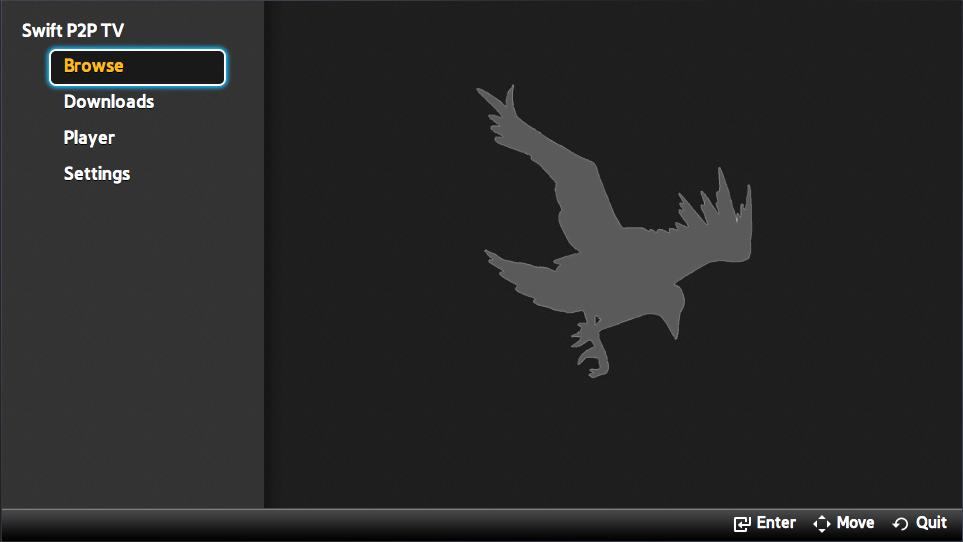
\includegraphics[width=1.2\textwidth]{Images/MainScene.jpg}}
	\caption{Screenshot of the Main scene.}
\end{figure}
\end{center}

\begin{center}
\begin{figure}[h]
	\centering
	\mbox{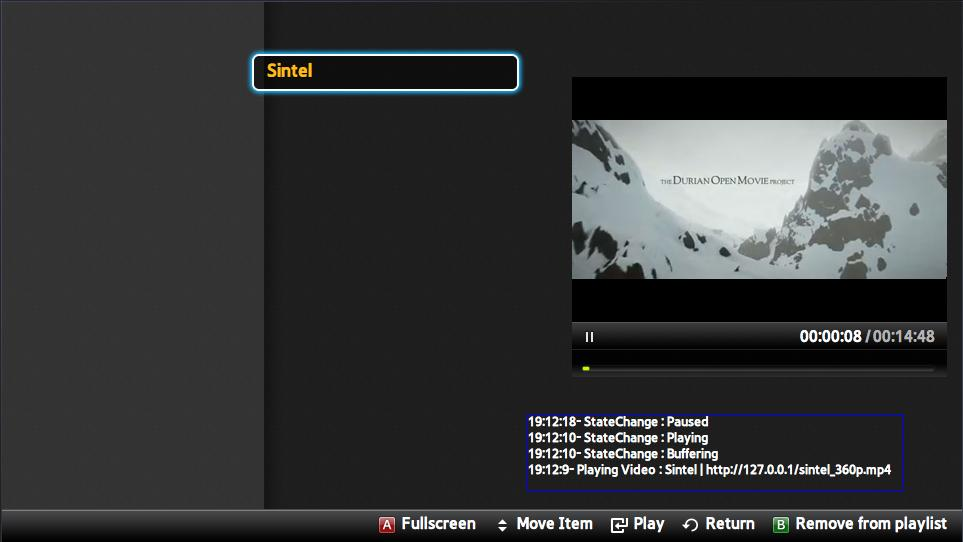
\includegraphics[width=1.2\textwidth]{Images/PlayerScene.jpg}}
	\caption{Screenshot of the Media Player scene.}
\end{figure}
\end{center}

\begin{center}
\begin{figure}[h]
	\centering
	\mbox{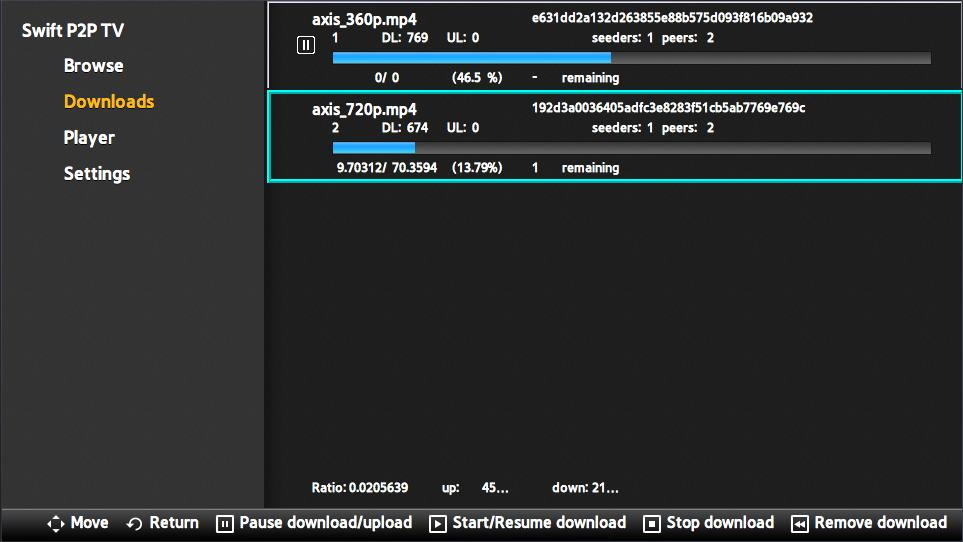
\includegraphics[width=1.2\textwidth]{Images/DownloadsScene.jpg}}
	\caption{Screenshot of the Downloads scene.}
\end{figure}
\end{center}

\begin{center}
\begin{figure}[h]
	\centering
	\mbox{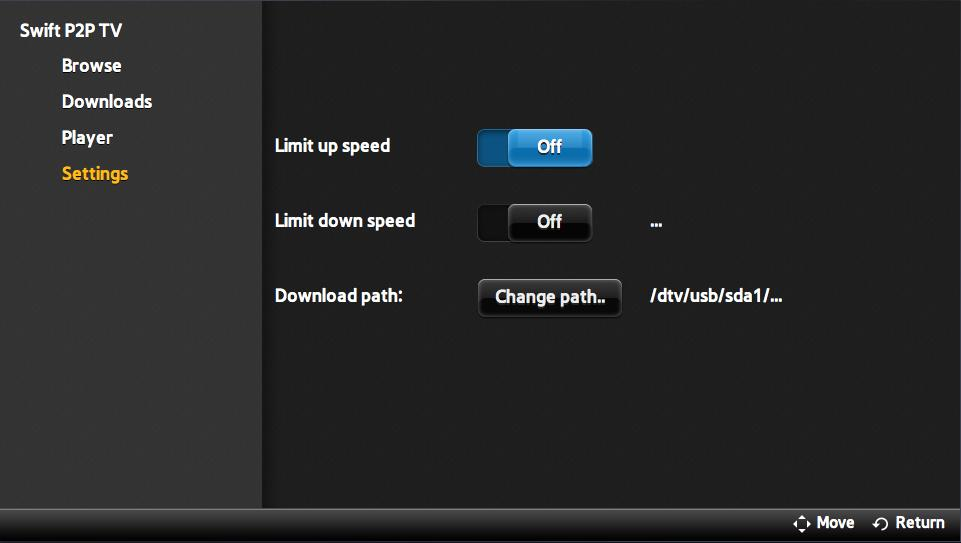
\includegraphics[width=1.2\textwidth]{Images/SettingsScene.jpg}}
	\caption{Screenshot of the Settings scene.}
\end{figure}
\end{center}

\chapter{Terms of reference}
\label{sec:terms}
\includepdf[pages={1-2}]{Images/terms.pdf}

\chapter{Orientation Report}
\label{sec:orientation}
\includepdf[pages={1-13}]{Images/orientation.pdf}

\chapter{Code API}
\label{sec:Doxygen}
\includepdf[pages={1-99}]{Images/refman.pdf}
